% DOPE 1.0 manuscript, preprint build. The body is dope1-content.tex; Figure 1 is dope1-hero.tex.
% Every result value is generated (paper/generated/dope1-*.tex, bench/real-world/render.py);
% a missing input typesets a visible [pending] marker instead of a number.
\documentclass[10pt,letterpaper]{article}
\usepackage[T1]{fontenc}
\usepackage[utf8]{inputenc}
\usepackage{mathptmx}
\usepackage[scaled=0.9]{helvet}
\usepackage{courier}
\usepackage[letterpaper,textwidth=6.1in,textheight=9in,centering]{geometry}
% Packages and environments shared by dope1.tex, dope1-supplement.tex and dope1-venue.tex.
% Class, fonts and page geometry are chosen by each wrapper.
\usepackage{amsmath,amssymb,amsthm}
\usepackage{booktabs}
\usepackage{graphicx}
\usepackage{xcolor}
\usepackage{caption}
\usepackage{enumitem}
\usepackage{microtype}
\usepackage{tikz}
\usetikzlibrary{positioning,arrows.meta}
\definecolor{stageline}{gray}{0.45}
\definecolor{stagefill}{gray}{0.975}
\definecolor{targetfill}{RGB}{233,241,251}
\definecolor{artfill}{RGB}{214,230,248}
\definecolor{arrowink}{gray}{0.4}
\newlength{\stageht}
\setlength{\stageht}{1.55cm}
\newlength{\stagewd}
\setlength{\stagewd}{2.55cm}
% A fixed-height text box for pipeline stages.
\newcommand{\stagebox}[2][\stagewd]{\parbox[c][\stageht][c]{#1}{\raggedright #2}}
% The venue class loads natbib itself (author-year); the preprint uses numbers.
\ifdefined\VenueBuild\else\usepackage[numbers,sort&compress]{natbib}\fi
\usepackage[colorlinks=true,linkcolor=linkblue,citecolor=linkblue,urlcolor=linkblue]{hyperref}
\usepackage[capitalise,noabbrev,nameinlink]{cleveref}
\definecolor{pendingcolor}{RGB}{176,58,46}
\definecolor{linkblue}{RGB}{31,86,160}
\captionsetup{font=small,labelfont=bf,skip=4pt}
\captionsetup[table]{position=top}

\theoremstyle{plain}
\newtheorem{theorem}{Theorem}
\newtheorem{proposition}[theorem]{Proposition}
\newtheorem{lemma}[theorem]{Lemma}
\newtheorem{corollary}[theorem]{Corollary}
\theoremstyle{definition}
\newtheorem{definition}[theorem]{Definition}
\theoremstyle{remark}
\newtheorem{remark}[theorem]{Remark}
% Algorithms are plain numbered floats (no texlive-science dependency).
\DeclareCaptionType[fileext=loa,placement=t]{algo}[Algorithm][List of Algorithms]
\crefname{algo}{Algorithm}{Algorithms}

% Shared macros for the TDL manuscript and supplement.
%
% Every number in the paper comes from paper/generated/ (claims firewall, T-070/T-071).
% generated/contract-macros.tex (paper/scripts/contract_macros.py from
% contracts/tdl-contract-v1.json; paper/build.sh refuses drift) and
% generated/headline-macros.tex (tools/claims/render.py from generated/headline-results.json)
% are read first when present; the contract file wins for the thresholds. The \providecommand defaults below are visible placeholders, so a
% missing generated file can never print a number that looks measured.
\IfFileExists{generated/contract-macros.tex}{% Generated by paper/scripts/contract_macros.py from contracts/tdl-contract-v1.json. Do not edit.
\newcommand{\MetricName}{TDL}
\newcommand{\ContractId}{tdl-contract-v1}
\newcommand{\ContractState}{draft (unfrozen)}
\newcommand{\HeadlinePoint}{T90/D80}
\newcommand{\TauT}{0.90}
\newcommand{\TauD}{0.80}
\newcommand{\ByteGrid}{0.5, 1, 2, 4, 8, 16, 32, 64, 128 and 256~KiB}
\newcommand{\SeedDesign}{five generator fit seeds by three sample seeds}
\newcommand{\BootstrapReplicates}{1{,}000}
\newcommand{\BootstrapSeed}{1729}
\newcommand{\LowerBoundLevel}{95\%}
\newcommand{\StabilityFloor}{0.70}
}{}
\IfFileExists{generated/headline-macros.tex}{% Generated by tools/claims/render.py; historical validation only.
\newcommand{\TdlMetricName}{TDL}
\newcommand{\TdlTransferThreshold}{0.90}
\newcommand{\TdlDriverThreshold}{0.80}
\newcommand{\HistoricalDopeRetention}{0.898}
\newcommand{\HistoricalDopeLower}{0.804}
\newcommand{\HistoricalDopeUpper}{0.972}
\newcommand{\HistoricalDopeBytes}{1895.0}
\newcommand{\HistoricalDopeLineages}{99}
\newcommand{\HistoricalDopeDefRetention}{0.704}
\newcommand{\HistoricalDopeDefLower}{0.424}
\newcommand{\HistoricalDopeDefUpper}{0.877}
\newcommand{\HistoricalDopeDefBytes}{1660.5}
\newcommand{\HistoricalDopeDefLineages}{99}
\newcommand{\HistoricalDopeHistRetention}{0.949}
\newcommand{\HistoricalDopeHistLower}{0.893}
\newcommand{\HistoricalDopeHistUpper}{0.987}
\newcommand{\HistoricalDopeHistLineages}{97}
\newcommand{\HistoricalDopeHistARetention}{0.801}
\newcommand{\HistoricalDopeHistALower}{0.445}
\newcommand{\HistoricalDopeHistAUpper}{0.958}
\newcommand{\HistoricalDopeHistALineages}{97}
\newcommand{\HistoricalDopeHistBRetention}{0.802}
\newcommand{\HistoricalDopeHistBLower}{0.457}
\newcommand{\HistoricalDopeHistBUpper}{0.958}
\newcommand{\HistoricalDopeHistBLineages}{93}
\newcommand{\HistoricalDopeHistCRetention}{0.931}
\newcommand{\HistoricalDopeHistCLower}{0.814}
\newcommand{\HistoricalDopeHistCUpper}{0.985}
\newcommand{\HistoricalDopeHistCLineages}{93}
\newcommand{\HistoricalDopeBnewRetention}{0.944}
\newcommand{\HistoricalDopeBnewLower}{0.893}
\newcommand{\HistoricalDopeBnewUpper}{0.985}
\newcommand{\HistoricalDopeBnewLineages}{99}
\newcommand{\HistoricalDopeBnewFourRetention}{0.862}
\newcommand{\HistoricalDopeBnewFourLower}{0.772}
\newcommand{\HistoricalDopeBnewFourUpper}{0.960}
\newcommand{\HistoricalDopeBnewFourLineages}{99}
\newcommand{\HistoricalTabSynRetention}{0.924}
\newcommand{\HistoricalTabSynLower}{0.814}
\newcommand{\HistoricalTabSynUpper}{0.965}
\newcommand{\HistoricalTabSynBytes}{42261045.5}
\newcommand{\HistoricalTabSynLineages}{99}
\newcommand{\HistoricalArfRetention}{0.822}
\newcommand{\HistoricalArfLower}{0.689}
\newcommand{\HistoricalArfUpper}{0.894}
\newcommand{\HistoricalArfBytes}{1438304.5}
\newcommand{\HistoricalArfLineages}{99}
\newcommand{\HistoricalArfNatRetention}{0.804}
\newcommand{\HistoricalArfNatLower}{0.647}
\newcommand{\HistoricalArfNatUpper}{0.885}
\newcommand{\HistoricalArfNatBytes}{1627718.5}
\newcommand{\HistoricalArfNatLineages}{99}
\newcommand{\HistoricalGaussRetention}{0.669}
\newcommand{\HistoricalGaussLower}{0.369}
\newcommand{\HistoricalGaussUpper}{0.867}
\newcommand{\HistoricalGaussBytes}{5464.5}
\newcommand{\HistoricalGaussLineages}{99}
\newcommand{\HistoricalChowRetention}{0.576}
\newcommand{\HistoricalChowLower}{0.294}
\newcommand{\HistoricalChowUpper}{0.638}
\newcommand{\HistoricalChowBytes}{29865.0}
\newcommand{\HistoricalChowLineages}{99}
\newcommand{\HistoricalIndRetention}{-0.012}
\newcommand{\HistoricalIndLower}{-0.040}
\newcommand{\HistoricalIndUpper}{-0.002}
\newcommand{\HistoricalIndBytes}{2549.5}
\newcommand{\HistoricalIndLineages}{99}
\newcommand{\HistoricalCtganRetention}{-0.080}
\newcommand{\HistoricalCtganLower}{-0.282}
\newcommand{\HistoricalCtganUpper}{0.223}
\newcommand{\HistoricalCtganBytes}{730999.0}
\newcommand{\HistoricalCtganLineages}{21}
\newcommand{\HistoricalTvaeRetention}{0.674}
\newcommand{\HistoricalTvaeLower}{0.452}
\newcommand{\HistoricalTvaeUpper}{0.776}
\newcommand{\HistoricalTvaeBytes}{308629.5}
\newcommand{\HistoricalTvaeLineages}{21}
\newcommand{\HistoricalCtganDefRetention}{-0.237}
\newcommand{\HistoricalCtganDefLower}{-0.509}
\newcommand{\HistoricalCtganDefUpper}{-0.022}
\newcommand{\HistoricalCtganDefLineages}{17}
\newcommand{\HistoricalTvaeDefRetention}{0.283}
\newcommand{\HistoricalTvaeDefLower}{0.175}
\newcommand{\HistoricalTvaeDefUpper}{0.596}
\newcommand{\HistoricalTvaeDefLineages}{18}
\newcommand{\HistoricalGaussDefRetention}{0.605}
\newcommand{\HistoricalGaussDefLower}{0.305}
\newcommand{\HistoricalGaussDefUpper}{0.879}
\newcommand{\HistoricalGaussDefLineages}{99}
\newcommand{\HistoricalChowDefRetention}{0.636}
\newcommand{\HistoricalChowDefLower}{0.545}
\newcommand{\HistoricalChowDefUpper}{0.754}
\newcommand{\HistoricalChowDefLineages}{99}
\newcommand{\HistoricalIndDefRetention}{-0.016}
\newcommand{\HistoricalIndDefLower}{-0.040}
\newcommand{\HistoricalIndDefUpper}{-0.006}
\newcommand{\HistoricalIndDefLineages}{99}
\newcommand{\HistoricalForestDefRetention}{1.011}
\newcommand{\HistoricalForestDefLower}{0.905}
\newcommand{\HistoricalForestDefUpper}{1.041}
\newcommand{\HistoricalForestDefLineages}{6}
\newcommand{\HistoricalForestRetention}{1.011}
\newcommand{\HistoricalForestLower}{0.905}
\newcommand{\HistoricalForestUpper}{1.041}
\newcommand{\HistoricalForestBytes}{325848913.5}
\newcommand{\HistoricalForestLineages}{6}
\newcommand{\HistoricalPredRetention}{0.631}
\newcommand{\HistoricalPredLower}{0.375}
\newcommand{\HistoricalPredUpper}{0.784}
\newcommand{\HistoricalPredLineages}{99}
\newcommand{\HistoricalPredSplitARetention}{0.600}
\newcommand{\HistoricalPredSplitALower}{0.365}
\newcommand{\HistoricalPredSplitAUpper}{0.778}
\newcommand{\HistoricalPredSplitALineages}{99}
\newcommand{\HistoricalPredSplitBRetention}{0.647}
\newcommand{\HistoricalPredSplitBLower}{0.368}
\newcommand{\HistoricalPredSplitBUpper}{0.777}
\newcommand{\HistoricalPredSplitBLineages}{100}
\newcommand{\HistoricalPredSplitCRetention}{0.640}
\newcommand{\HistoricalPredSplitCLower}{0.362}
\newcommand{\HistoricalPredSplitCUpper}{0.777}
\newcommand{\HistoricalPredSplitCLineages}{100}
\newcommand{\HistoricalPredSplitDRetention}{0.677}
\newcommand{\HistoricalPredSplitDLower}{0.359}
\newcommand{\HistoricalPredSplitDUpper}{0.787}
\newcommand{\HistoricalPredSplitDLineages}{100}
\newcommand{\HistoricalBootRetention}{1.018}
\newcommand{\HistoricalBootLower}{1.005}
\newcommand{\HistoricalBootUpper}{1.028}
\newcommand{\HistoricalBootLineages}{99}
}{}

\newcommand{\pending}[1]{\textcolor{pendingcolor}{\textbf{[#1]}}}
% Names emitted by tools/claims/render.py (L2) take precedence over the placeholders.
\ifdefined\TdlMetricName\providecommand{\MetricName}{\TdlMetricName}\fi
\ifdefined\TdlTransferThreshold\providecommand{\TauT}{\TdlTransferThreshold}\fi
\ifdefined\TdlDriverThreshold\providecommand{\TauD}{\TdlDriverThreshold}\fi
\providecommand{\MetricName}{TDL}
\providecommand{\MetricLong}{Transfer Description Length}
\providecommand{\TauT}{\pending{$\tau_T$ from contract}}
\providecommand{\TauD}{\pending{$\tau_D$ from contract}}
\providecommand{\HeadlinePoint}{\pending{headline operating point}}
\providecommand{\ByteGrid}{\pending{byte grid from contract}}
\providecommand{\SeedDesign}{\pending{seed design from contract}}
\providecommand{\ResultStatus}{specified, not measured}

% Display helpers.
\newcommand{\Lnull}{L_{\mathrm{null}}}
\newcommand{\Lreal}{L_{\mathrm{real}}}
\newcommand{\Lsyn}{L_{\mathrm{syn}}}
\newcommand{\Trobust}{T_{\mathrm{robust}}}
\newcommand{\Drobust}{D_{\mathrm{robust}}}
\newcommand{\LCB}{\operatorname{LCB}_{1-\alpha}}

% Generated inputs with placeholders when absent.
\newlength{\pendingwidth}
\setlength{\pendingwidth}{0.9\linewidth}
\newlength{\herowidth}
\setlength{\herowidth}{0.86\linewidth}
% Figure 1 (compression frontier) and the foundation-model figure in the main text.
\newlength{\frontierwidth}
\setlength{\frontierwidth}{0.9\linewidth}
\newlength{\foundationwidth}
\setlength{\foundationwidth}{0.62\linewidth}
\newcommand{\GeneratedFigure}[3][\linewidth]{%
  \IfFileExists{generated/#2}{\includegraphics[width=#1]{generated/#2}}{%
    \fbox{\parbox{\pendingwidth}{\centering\vspace{2em}\pending{#3}\vspace{2em}}}}}
\newcommand{\GeneratedTable}[2]{%
  \IfFileExists{generated/#1}{\input{generated/#1}}{%
    \fbox{\parbox{\pendingwidth}{\centering\vspace{1em}\pending{#2}\vspace{1em}}}}}
% \Hist{Dope}{Retention} prints \HistoricalDopeRetention from headline-macros.tex, or a placeholder.
\newcommand{\Hist}[2]{\ifcsname Historical#1#2\endcsname\csname Historical#1#2\endcsname\else\pending{generated}\fi}
\newcommand{\HistRow}[2]{#2 & \Hist{#1}{Retention} [\Hist{#1}{Lower}, \Hist{#1}{Upper}] & \Hist{#1}{Lineages}}

% DOPE 1.0 engine benchmark (bench/real-world/render.py): results and source-derived settings.
\IfFileExists{generated/dope1-macros.tex}{% Generated by bench/real-world/render.py from summary.json; do not edit.
\newcommand{\OneTables}{16}
\newcommand{\OneArfN}{16}
\newcommand{\OneArfRet}{0.705}
\newcommand{\OneArfLo}{0.000}
\newcommand{\OneArfHi}{0.856}
\newcommand{\OneArfBytes}{673.1~KiB}
\newcommand{\OneArfReach}{3}
\newcommand{\OneArfFit}{30.2~s}
\newcommand{\OneArfRate}{3k}
\newcommand{\OneArfCb}{0.847}
\newcommand{\OneArfLin}{0.945}
\newcommand{\OneArfMlp}{0.849}
\newcommand{\OneBootN}{16}
\newcommand{\OneBootRet}{0.929}
\newcommand{\OneBootLo}{0.669}
\newcommand{\OneBootHi}{0.988}
\newcommand{\OneBootBytes}{52.1~KiB}
\newcommand{\OneBootReach}{9}
\newcommand{\OneBootCb}{0.973}
\newcommand{\OneBootLin}{0.996}
\newcommand{\OneBootMlp}{0.961}
\newcommand{\OneCopulaN}{16}
\newcommand{\OneCopulaRet}{0.282}
\newcommand{\OneCopulaLo}{0.094}
\newcommand{\OneCopulaHi}{0.447}
\newcommand{\OneCopulaBytes}{82.0~KiB}
\newcommand{\OneCopulaReach}{1}
\newcommand{\OneCopulaFit}{4.7~s}
\newcommand{\OneCopulaRate}{21k}
\newcommand{\OneCopulaCb}{0.400}
\newcommand{\OneCopulaLin}{0.759}
\newcommand{\OneCopulaMlp}{0.288}
\newcommand{\OneCtganN}{7}
\newcommand{\OneCtganRet}{\ensuremath{-}1.897}
\newcommand{\OneCtganLo}{\ensuremath{-}3.060}
\newcommand{\OneCtganHi}{\ensuremath{-}0.473}
\newcommand{\OneCtganBytes}{712.9~KiB}
\newcommand{\OneCtganReach}{0}
\newcommand{\OneCtganFit}{5~min}
\newcommand{\OneCtganRate}{3k}
\newcommand{\OneCtganCb}{\ensuremath{-}0.389}
\newcommand{\OneCtganLin}{\ensuremath{-}0.181}
\newcommand{\OneCtganMlp}{\ensuremath{-}2.331}
\newcommand{\OneDopeEN}{16}
\newcommand{\OneDopeERet}{0.933}
\newcommand{\OneDopeELo}{0.869}
\newcommand{\OneDopeEHi}{0.965}
\newcommand{\OneDopeEBytes}{5.7~KiB}
\newcommand{\OneDopeEReach}{10}
\newcommand{\OneDopeEFit}{14.9~s}
\newcommand{\OneDopeERate}{80k}
\newcommand{\OneDopeECb}{0.947}
\newcommand{\OneDopeELin}{0.956}
\newcommand{\OneDopeEMlp}{0.955}
\newcommand{\OneDopeAN}{16}
\newcommand{\OneDopeARet}{0.722}
\newcommand{\OneDopeALo}{0.165}
\newcommand{\OneDopeAHi}{0.891}
\newcommand{\OneDopeABytes}{1012~B}
\newcommand{\OneDopeAReach}{4}
\newcommand{\OneDopeAFit}{8.5~s}
\newcommand{\OneDopeARate}{173k}
\newcommand{\OneDopeACb}{0.875}
\newcommand{\OneDopeALin}{0.956}
\newcommand{\OneDopeAMlp}{0.895}
\newcommand{\OneDopeBN}{16}
\newcommand{\OneDopeBRet}{0.905}
\newcommand{\OneDopeBLo}{0.815}
\newcommand{\OneDopeBHi}{0.939}
\newcommand{\OneDopeBBytes}{2.0~KiB}
\newcommand{\OneDopeBReach}{8}
\newcommand{\OneDopeBFit}{12.9~s}
\newcommand{\OneDopeBRate}{141k}
\newcommand{\OneDopeBCb}{0.925}
\newcommand{\OneDopeBLin}{0.941}
\newcommand{\OneDopeBMlp}{0.939}
\newcommand{\OneDopeCN}{16}
\newcommand{\OneDopeCRet}{0.909}
\newcommand{\OneDopeCLo}{0.843}
\newcommand{\OneDopeCHi}{0.932}
\newcommand{\OneDopeCBytes}{3.8~KiB}
\newcommand{\OneDopeCReach}{9}
\newcommand{\OneDopeCFit}{12.4~s}
\newcommand{\OneDopeCRate}{116k}
\newcommand{\OneDopeCCb}{0.937}
\newcommand{\OneDopeCLin}{0.964}
\newcommand{\OneDopeCMlp}{0.933}
\newcommand{\OneDopeFN}{16}
\newcommand{\OneDopeFRet}{0.930}
\newcommand{\OneDopeFLo}{0.878}
\newcommand{\OneDopeFHi}{0.960}
\newcommand{\OneDopeFBytes}{9.6~KiB}
\newcommand{\OneDopeFReach}{11}
\newcommand{\OneDopeFFit}{18.6~s}
\newcommand{\OneDopeFRate}{44k}
\newcommand{\OneDopeFCb}{0.954}
\newcommand{\OneDopeFLin}{0.959}
\newcommand{\OneDopeFMlp}{0.967}
\newcommand{\OneDopeDN}{16}
\newcommand{\OneDopeDRet}{0.939}
\newcommand{\OneDopeDLo}{0.849}
\newcommand{\OneDopeDHi}{0.961}
\newcommand{\OneDopeDBytes}{4.3~KiB}
\newcommand{\OneDopeDReach}{11}
\newcommand{\OneDopeDFit}{12.0~s}
\newcommand{\OneDopeDRate}{124k}
\newcommand{\OneDopeDCb}{0.943}
\newcommand{\OneDopeDLin}{0.956}
\newcommand{\OneDopeDMlp}{0.961}
\newcommand{\OneDopeOneRegimeN}{16}
\newcommand{\OneDopeOneRegimeRet}{0.835}
\newcommand{\OneDopeOneRegimeLo}{0.758}
\newcommand{\OneDopeOneRegimeHi}{0.928}
\newcommand{\OneDopeOneRegimeBytes}{3.4~KiB}
\newcommand{\OneDopeOneRegimeReach}{7}
\newcommand{\OneDopeOneRegimeFit}{8.5~s}
\newcommand{\OneDopeOneRegimeRate}{133k}
\newcommand{\OneDopeOneRegimeCb}{0.921}
\newcommand{\OneDopeOneRegimeLin}{0.908}
\newcommand{\OneDopeOneRegimeMlp}{0.928}
\newcommand{\OneDopeFourN}{16}
\newcommand{\OneDopeFourRet}{0.944}
\newcommand{\OneDopeFourLo}{0.813}
\newcommand{\OneDopeFourHi}{0.955}
\newcommand{\OneDopeFourBytes}{3.8~KiB}
\newcommand{\OneDopeFourReach}{10}
\newcommand{\OneDopeFourFit}{11.1~s}
\newcommand{\OneDopeFourRate}{187k}
\newcommand{\OneDopeFourCb}{0.965}
\newcommand{\OneDopeFourLin}{0.955}
\newcommand{\OneDopeFourMlp}{0.974}
\newcommand{\OneDopeIndepN}{16}
\newcommand{\OneDopeIndepRet}{0.798}
\newcommand{\OneDopeIndepLo}{0.536}
\newcommand{\OneDopeIndepHi}{0.892}
\newcommand{\OneDopeIndepBytes}{3.3~KiB}
\newcommand{\OneDopeIndepReach}{4}
\newcommand{\OneDopeIndepFit}{8.7~s}
\newcommand{\OneDopeIndepRate}{168k}
\newcommand{\OneDopeIndepCb}{0.890}
\newcommand{\OneDopeIndepLin}{0.855}
\newcommand{\OneDopeIndepMlp}{0.923}
\newcommand{\OneDopeLinearN}{16}
\newcommand{\OneDopeLinearRet}{0.593}
\newcommand{\OneDopeLinearLo}{0.370}
\newcommand{\OneDopeLinearHi}{0.798}
\newcommand{\OneDopeLinearBytes}{1.0~KiB}
\newcommand{\OneDopeLinearReach}{3}
\newcommand{\OneDopeLinearFit}{2.9~s}
\newcommand{\OneDopeLinearRate}{207k}
\newcommand{\OneDopeLinearCb}{0.621}
\newcommand{\OneDopeLinearLin}{0.959}
\newcommand{\OneDopeLinearMlp}{0.767}
\newcommand{\OneDopeNoAuditN}{16}
\newcommand{\OneDopeNoAuditRet}{0.919}
\newcommand{\OneDopeNoAuditLo}{0.832}
\newcommand{\OneDopeNoAuditHi}{0.949}
\newcommand{\OneDopeNoAuditBytes}{3.8~KiB}
\newcommand{\OneDopeNoAuditReach}{9}
\newcommand{\OneDopeNoAuditFit}{10.1~s}
\newcommand{\OneDopeNoAuditRate}{126k}
\newcommand{\OneDopeNoAuditCb}{0.950}
\newcommand{\OneDopeNoAuditLin}{0.948}
\newcommand{\OneDopeNoAuditMlp}{0.961}
\newcommand{\OneDopeNoTreesN}{16}
\newcommand{\OneDopeNoTreesRet}{0.862}
\newcommand{\OneDopeNoTreesLo}{0.774}
\newcommand{\OneDopeNoTreesHi}{0.937}
\newcommand{\OneDopeNoTreesBytes}{1.6~KiB}
\newcommand{\OneDopeNoTreesReach}{6}
\newcommand{\OneDopeNoTreesFit}{9.5~s}
\newcommand{\OneDopeNoTreesRate}{152k}
\newcommand{\OneDopeNoTreesCb}{0.884}
\newcommand{\OneDopeNoTreesLin}{0.979}
\newcommand{\OneDopeNoTreesMlp}{0.930}
\newcommand{\OneDopeSeedZeroN}{16}
\newcommand{\OneDopeSeedZeroRet}{0.919}
\newcommand{\OneDopeSeedZeroLo}{0.832}
\newcommand{\OneDopeSeedZeroHi}{0.949}
\newcommand{\OneDopeSeedZeroBytes}{3.8~KiB}
\newcommand{\OneDopeSeedZeroReach}{9}
\newcommand{\OneDopeSeedZeroFit}{12.5~s}
\newcommand{\OneDopeSeedZeroRate}{123k}
\newcommand{\OneDopeSeedZeroCb}{0.950}
\newcommand{\OneDopeSeedZeroLin}{0.948}
\newcommand{\OneDopeSeedZeroMlp}{0.961}
\newcommand{\OneKernelN}{16}
\newcommand{\OneKernelRet}{0.677}
\newcommand{\OneKernelLo}{0.484}
\newcommand{\OneKernelHi}{0.844}
\newcommand{\OneKernelBytes}{1.1~KiB}
\newcommand{\OneKernelReach}{3}
\newcommand{\OneKernelFit}{4.9~s}
\newcommand{\OneKernelRate}{162k}
\newcommand{\OneKernelCb}{0.794}
\newcommand{\OneKernelLin}{0.955}
\newcommand{\OneKernelMlp}{0.824}
\newcommand{\OneRowsEN}{16}
\newcommand{\OneRowsERet}{0.872}
\newcommand{\OneRowsELo}{\ensuremath{-}0.942}
\newcommand{\OneRowsEHi}{0.998}
\newcommand{\OneRowsEBytes}{16.0~KiB}
\newcommand{\OneRowsEReach}{7}
\newcommand{\OneRowsECb}{0.972}
\newcommand{\OneRowsELin}{0.989}
\newcommand{\OneRowsEMlp}{0.872}
\newcommand{\OneRowsAN}{16}
\newcommand{\OneRowsARet}{\ensuremath{-}0.409}
\newcommand{\OneRowsALo}{\ensuremath{-}2.174}
\newcommand{\OneRowsAHi}{0.279}
\newcommand{\OneRowsABytes}{1020~B}
\newcommand{\OneRowsAReach}{1}
\newcommand{\OneRowsACb}{0.538}
\newcommand{\OneRowsALin}{0.650}
\newcommand{\OneRowsAMlp}{\ensuremath{-}0.437}
\newcommand{\OneRowsBN}{16}
\newcommand{\OneRowsBRet}{\ensuremath{-}0.286}
\newcommand{\OneRowsBLo}{\ensuremath{-}3.975}
\newcommand{\OneRowsBHi}{0.519}
\newcommand{\OneRowsBBytes}{2.0~KiB}
\newcommand{\OneRowsBReach}{3}
\newcommand{\OneRowsBCb}{0.788}
\newcommand{\OneRowsBLin}{0.870}
\newcommand{\OneRowsBMlp}{\ensuremath{-}0.248}
\newcommand{\OneRowsCN}{16}
\newcommand{\OneRowsCRet}{0.340}
\newcommand{\OneRowsCLo}{\ensuremath{-}4.012}
\newcommand{\OneRowsCHi}{0.918}
\newcommand{\OneRowsCBytes}{4.0~KiB}
\newcommand{\OneRowsCReach}{5}
\newcommand{\OneRowsCCb}{0.871}
\newcommand{\OneRowsCLin}{0.937}
\newcommand{\OneRowsCMlp}{0.376}
\newcommand{\OneRowsFN}{16}
\newcommand{\OneRowsFRet}{0.983}
\newcommand{\OneRowsFLo}{0.950}
\newcommand{\OneRowsFHi}{0.998}
\newcommand{\OneRowsFBytes}{50.8~KiB}
\newcommand{\OneRowsFReach}{12}
\newcommand{\OneRowsFCb}{0.996}
\newcommand{\OneRowsFLin}{1.000}
\newcommand{\OneRowsFMlp}{0.984}
\newcommand{\OneRowsDN}{16}
\newcommand{\OneRowsDRet}{0.564}
\newcommand{\OneRowsDLo}{\ensuremath{-}3.908}
\newcommand{\OneRowsDHi}{0.986}
\newcommand{\OneRowsDBytes}{8.0~KiB}
\newcommand{\OneRowsDReach}{7}
\newcommand{\OneRowsDCb}{0.924}
\newcommand{\OneRowsDLin}{0.980}
\newcommand{\OneRowsDMlp}{0.564}
\newcommand{\OneRowsFullN}{16}
\newcommand{\OneRowsFullRet}{0.999}
\newcommand{\OneRowsFullLo}{0.996}
\newcommand{\OneRowsFullHi}{1.000}
\newcommand{\OneRowsFullBytes}{52.2~KiB}
\newcommand{\OneRowsFullReach}{16}
\newcommand{\OneRowsFullCb}{0.999}
\newcommand{\OneRowsFullLin}{1.000}
\newcommand{\OneRowsFullMlp}{1.001}
\newcommand{\OneTvaeN}{7}
\newcommand{\OneTvaeRet}{\ensuremath{-}0.460}
\newcommand{\OneTvaeLo}{\ensuremath{-}1.361}
\newcommand{\OneTvaeHi}{0.611}
\newcommand{\OneTvaeBytes}{247.7~KiB}
\newcommand{\OneTvaeReach}{0}
\newcommand{\OneTvaeFit}{83.5~s}
\newcommand{\OneTvaeRate}{5k}
\newcommand{\OneTvaeCb}{0.398}
\newcommand{\OneTvaeLin}{0.735}
\newcommand{\OneTvaeMlp}{\ensuremath{-}0.533}
\newcommand{\OneDiffArf}{+0.441}
\newcommand{\OneDiffArfLo}{+0.110}
\newcommand{\OneDiffArfHi}{+0.644}
\newcommand{\OneDiffArfWtl}{15/0/1}
\newcommand{\OneDiffBoot}{\ensuremath{-}0.028}
\newcommand{\OneDiffBootLo}{\ensuremath{-}0.090}
\newcommand{\OneDiffBootHi}{+0.770}
\newcommand{\OneDiffBootWtl}{5/0/11}
\newcommand{\OneDiffCopula}{+0.644}
\newcommand{\OneDiffCopulaLo}{+0.390}
\newcommand{\OneDiffCopulaHi}{+2.856}
\newcommand{\OneDiffCopulaWtl}{15/0/1}
\newcommand{\OneDiffCtgan}{+2.790}
\newcommand{\OneDiffCtganLo}{+1.139}
\newcommand{\OneDiffCtganHi}{+4.214}
\newcommand{\OneDiffCtganWtl}{7/0/0}
\newcommand{\OneDiffDopeOneRegime}{+0.035}
\newcommand{\OneDiffDopeOneRegimeLo}{\ensuremath{-}0.017}
\newcommand{\OneDiffDopeOneRegimeHi}{+0.070}
\newcommand{\OneDiffDopeOneRegimeWtl}{11/0/5}
\newcommand{\OneDiffDopeFour}{\ensuremath{-}0.021}
\newcommand{\OneDiffDopeFourLo}{\ensuremath{-}0.065}
\newcommand{\OneDiffDopeFourHi}{+0.007}
\newcommand{\OneDiffDopeFourWtl}{4/0/12}
\newcommand{\OneDiffDopeIndep}{+0.137}
\newcommand{\OneDiffDopeIndepLo}{+0.031}
\newcommand{\OneDiffDopeIndepHi}{+0.248}
\newcommand{\OneDiffDopeIndepWtl}{12/0/4}
\newcommand{\OneDiffDopeLinear}{+0.242}
\newcommand{\OneDiffDopeLinearLo}{+0.136}
\newcommand{\OneDiffDopeLinearHi}{+0.422}
\newcommand{\OneDiffDopeLinearWtl}{14/0/2}
\newcommand{\OneDiffDopeNoAudit}{\ensuremath{-}0.003}
\newcommand{\OneDiffDopeNoAuditLo}{\ensuremath{-}0.018}
\newcommand{\OneDiffDopeNoAuditHi}{+0.135}
\newcommand{\OneDiffDopeNoAuditWtl}{3/4/9}
\newcommand{\OneDiffDopeNoTrees}{+0.043}
\newcommand{\OneDiffDopeNoTreesLo}{\ensuremath{-}0.008}
\newcommand{\OneDiffDopeNoTreesHi}{+0.199}
\newcommand{\OneDiffDopeNoTreesWtl}{13/0/3}
\newcommand{\OneDiffKernel}{+0.205}
\newcommand{\OneDiffKernelLo}{+0.070}
\newcommand{\OneDiffKernelHi}{+0.388}
\newcommand{\OneDiffKernelWtl}{13/0/3}
\newcommand{\OneDiffRowsC}{+1.578}
\newcommand{\OneDiffRowsCLo}{+0.218}
\newcommand{\OneDiffRowsCHi}{+10.708}
\newcommand{\OneDiffRowsCWtl}{11/0/5}
\newcommand{\OneDiffRowsFull}{\ensuremath{-}0.109}
\newcommand{\OneDiffRowsFullLo}{\ensuremath{-}0.271}
\newcommand{\OneDiffRowsFullHi}{\ensuremath{-}0.067}
\newcommand{\OneDiffRowsFullWtl}{0/0/16}
\newcommand{\OneDiffTvae}{+1.374}
\newcommand{\OneDiffTvaeLo}{+0.609}
\newcommand{\OneDiffTvaeHi}{+327.804}
\newcommand{\OneDiffTvaeWtl}{7/0/0}
\newcommand{\OneEqEWtl}{10/0/6}
\newcommand{\OneEqEP}{0.45}
\newcommand{\OneEqEN}{16}
\newcommand{\OneEqAWtl}{11/0/1}
\newcommand{\OneEqAP}{0.0063}
\newcommand{\OneEqAN}{12}
\newcommand{\OneEqBWtl}{14/0/2}
\newcommand{\OneEqBP}{0.0042}
\newcommand{\OneEqBN}{16}
\newcommand{\OneEqCWtl}{11/0/5}
\newcommand{\OneEqCP}{0.21}
\newcommand{\OneEqCN}{16}
\newcommand{\OneEqFWtl}{4/0/12}
\newcommand{\OneEqFP}{0.077}
\newcommand{\OneEqFN}{16}
\newcommand{\OneEqDWtl}{10/0/6}
\newcommand{\OneEqDP}{0.45}
\newcommand{\OneEqDN}{16}
\newcommand{\OneKernelSupported}{14}
\newcommand{\OneKernelUnsupported}{2}
\newcommand{\OneKernelVsAWtl}{9/0/5}
\newcommand{\OneKernelVsAHl}{+0.010}
\newcommand{\OneKernelVsALo}{\ensuremath{-}0.394}
\newcommand{\OneKernelVsAHi}{+0.126}
\newcommand{\OneKernelVsAP}{0.42}
\newcommand{\OneKernelVsAN}{14}
\newcommand{\OneKernelVsBWtl}{12/0/2}
\newcommand{\OneKernelVsBHl}{+0.166}
\newcommand{\OneKernelVsBLo}{+0.047}
\newcommand{\OneKernelVsBHi}{+0.291}
\newcommand{\OneKernelVsBP}{0.013}
\newcommand{\OneKernelVsBN}{14}
\newcommand{\OneKernelVsCWtl}{11/0/3}
\newcommand{\OneKernelVsCHl}{+0.160}
\newcommand{\OneKernelVsCLo}{+0.045}
\newcommand{\OneKernelVsCHi}{+0.306}
\newcommand{\OneKernelVsCP}{0.057}
\newcommand{\OneKernelVsCN}{14}
\newcommand{\OneAuditN}{124}
\newcommand{\OneAuditRho}{0.73}
\newcommand{\OneAuditMae}{0.042}
\newcommand{\OneAuditBias}{\ensuremath{-}0.006}
\newcommand{\OneAblDopeOneRegimeWtl}{4/1/11}
\newcommand{\OneAblDopeOneRegimeP}{0.12}
\newcommand{\OneAblDopeFourWtl}{11/0/5}
\newcommand{\OneAblDopeFourP}{0.21}
\newcommand{\OneAblDopeIndepWtl}{4/0/12}
\newcommand{\OneAblDopeIndepP}{0.077}
\newcommand{\OneAblDopeLinearWtl}{3/0/13}
\newcommand{\OneAblDopeLinearP}{0.021}
\newcommand{\OneAblDopeNoAuditWtl}{1/14/1}
\newcommand{\OneAblDopeNoAuditP}{1}
\newcommand{\OneAblDopeNoTreesWtl}{1/0/15}
\newcommand{\OneAblDopeNoTreesP}{0.00052}
\newcommand{\OneEqBudgets}{6}
\newcommand{\OneEqWins}{60}
\newcommand{\OneEqLosses}{32}
\newcommand{\OneEqCells}{92}
\newcommand{\OneDopeFailedE}{0}
\newcommand{\OneDopeFailedA}{4}
\newcommand{\OneDopeFailedB}{0}
\newcommand{\OneDopeFailedC}{0}
\newcommand{\OneDopeFailedF}{0}
\newcommand{\OneDopeFailedD}{0}
\newcommand{\OneTdlDopeN}{11}
\newcommand{\OneTdlDopeMedian}{1.9~KiB}
\newcommand{\OneTdlRowsN}{16}
\newcommand{\OneTdlRowsMedian}{50.8~KiB}
\newcommand{\OneTdlDopeEightyN}{13}
\newcommand{\OneTdlDopeEightyMedian}{1.9~KiB}
\newcommand{\OneTdlRowsEightyN}{16}
\newcommand{\OneTdlRowsEightyMedian}{16.0~KiB}
\newcommand{\MlcVTwoDatasets}{1{,}000}
\newcommand{\MlcVTwoTrainLossInit}{0.42415}
\newcommand{\MlcVTwoTrainLossBest}{0.36193}
\newcommand{\MlcVTwoTrainLossFinal}{0.36201}
\newcommand{\MlcVTwoLossInit}{0.43934}
\newcommand{\MlcVTwoLossBest}{0.37667}
\newcommand{\MlcVTwoLossFinal}{0.37686}
\newcommand{\MlcVTwoFullValLoss}{0.37753}
\newcommand{\MlcVTwoValMedBest}{0.39900}
\newcommand{\MlcVTwoValHighBest}{0.37377}
\newcommand{\MlcVTwoValUltraBest}{0.35725}
\newcommand{\MlcVTwoFullValMed}{0.39744}
\newcommand{\MlcVTwoFullValHigh}{0.37456}
\newcommand{\MlcVTwoFullValUltra}{0.36060}
\newcommand{\MlcMaxTrainValDsFrac}{3.61\%}
\newcommand{\MlcMaxTrainValSplitFrac}{3.59\%}
\newcommand{\MlcMaxTrainTrainSplitFrac}{96.41\%}
\newcommand{\MlcMaxTrainValSplits}{684}
\newcommand{\MlcMaxTrainTrainSplits}{18{,}395}
\newcommand{\MlcMaxTrainVisits}{24{,}527}
\newcommand{\MlcMaxTrainEffPasses}{1.333351}
\newcommand{\MlcMaxTrainLossInit}{0.40988}
\newcommand{\MlcMaxTrainLossInitSe}{0.01767}
\newcommand{\MlcMaxTrainLossBest}{0.34216}
\newcommand{\MlcMaxTrainLossBestSe}{0.01621}
\newcommand{\MlcMaxTrainLossDropPct}{16.52\%}
\newcommand{\MlcMaxTrainTrainInit}{0.41216}
\newcommand{\MlcMaxTrainTrainBest}{0.35175}
\newcommand{\MlcMaxTrainValMedBest}{0.36407}
\newcommand{\MlcMaxTrainValHighBest}{0.33844}
\newcommand{\MlcMaxTrainValUltraBest}{0.32396}
\newcommand{\MlcDisjointValDsFrac}{2.82\%}
\newcommand{\MlcDisjointValSplitFrac}{2.80\%}
\newcommand{\MlcDisjointTrainSplitFrac}{97.20\%}
\newcommand{\MlcDisjointVisits}{15{,}968}
\newcommand{\MlcDisjointEffPasses}{1.333333}
\newcommand{\MlcDisjointLossInit}{0.60691}
\newcommand{\MlcDisjointLossInitSe}{0.01915}
\newcommand{\MlcDisjointLossBest}{0.57363}
\newcommand{\MlcDisjointLossBestSe}{0.02131}
\newcommand{\MlcDisjointLossFinal}{0.57371}
\newcommand{\MlcDisjointLossFinalSe}{0.02074}
\newcommand{\MlcDisjointTrainInit}{0.47854}
\newcommand{\MlcDisjointTrainBest}{0.41521}
\newcommand{\MlcDisjointTrainFinal}{0.41492}
\newcommand{\MlcVThreeMaxTrainLoadedTrain}{2{,}229}
\newcommand{\MlcVThreeMaxTrainLoadedVal}{75}
\newcommand{\MlcVThreeMaxTrainLoadedPool}{2{,}304}
\newcommand{\MlcVThreeMaxTrainLoadedValFrac}{3.26\%}
\newcommand{\MlcVThreeMaxTrainLoadedTrainFrac}{96.74\%}
\newcommand{\MlcVThreeMaxTrainCatalogValFrac}{3.29\%}
\newcommand{\MlcVThreeMaxTrainVisits}{4{,}457}
\newcommand{\MlcVThreeMaxTrainEffPasses}{1.999551}
\newcommand{\MlcVThreeMaxTrainLossInit}{0.69727}
\newcommand{\MlcVThreeMaxTrainLossInitSe}{0.03888}
\newcommand{\MlcVThreeMaxTrainLossBest}{0.68492}
\newcommand{\MlcVThreeMaxTrainLossBestSe}{0.03877}
\newcommand{\MlcVThreeMaxTrainAZeroBest}{0.68700}
\newcommand{\MlcVThreeMaxTrainAOneBest}{0.68531}
\newcommand{\MlcVThreeMaxTrainATwoBest}{0.68489}
\newcommand{\MlcVTwoPooledElo}{1651.3}
\newcommand{\MlcVTwoDisjointElo}{1650.7}
\newcommand{\MlcVTwoHeldoutElo}{1671.1}
\newcommand{\MlcVTwoUltraR}{0.8975}
\newcommand{\MlcVTwoUltraRMed}{0.9658}
\newcommand{\MlcVTwoUltraD}{0.7896}
\newcommand{\MlcVThreeDatasets}{1{,}069}
\newcommand{\MlcVThreeCells}{4{,}276}
\newcommand{\MlcVThreeLossAZero}{0.83084}
\newcommand{\MlcVThreeLossAThree}{0.82748}
\newcommand{\MlcVThreeDriverLossAZero}{0.04205}
\newcommand{\MlcVThreeDriverLossAThree}{0.03954}
\newcommand{\MlcVThreeMcHighR}{0.8402}
\newcommand{\MlcVThreeMcHighCscR}{0.8451}
\newcommand{\MlcVThreePanelHighR}{0.8633}
\newcommand{\MlcVThreePanelHighCscR}{0.8706}
\newcommand{\MlcVThreeElo}{1457.6}
\newcommand{\MlcVThreeCopulaDeltaR}{+0.0941}
\newcommand{\MlcVThreeMcCopulaDeltaR}{+0.2526}
\newcommand{\MlcRustParams}{444{,}168}
\newcommand{\MlcRustFwdErr}{1.3255e-6}
\newcommand{\MlcRustSampleErr}{1.1111e-6}
}{}
\IfFileExists{generated/dope1-config.tex}{% Generated by bench/real-world/render.py from engine and harness sources; do not edit.
\newcommand{\CfgBudget}{4}
\newcommand{\CfgZGrid}{3}
\newcommand{\CfgMaxDiscrete}{24}
\newcommand{\CfgResidualKnots}{9}
\newcommand{\CfgAtomShare}{10}
\newcommand{\CfgMaxRegimes}{16}
\newcommand{\CfgRegimeLadder}{1,2,3,4,6,8,12,16}
\newcommand{\CfgSteps}{1500}
\newcommand{\CfgLearningRate}{$10^{-2}$}
\newcommand{\CfgWeightDecay}{$10^{-4}$}
\newcommand{\CfgBatch}{2048}
\newcommand{\CfgEvalEvery}{50}
\newcommand{\CfgPatience}{400}
\newcommand{\CfgTolerance}{0.5}
\newcommand{\CfgReadoutRows}{8192}
\newcommand{\CfgScoreTable}{257}
\newcommand{\CfgMinLevel}{5}
\newcommand{\CfgMaxLevels}{64}
\newcommand{\CfgLevels}{256}
\newcommand{\CfgMaxTrees}{1500}
\newcommand{\CfgLeafBits}{6}
\newcommand{\CfgShares}{5, 15, 30}
\newcommand{\CfgAuditRows}{6000}
\newcommand{\CfgMaxTrain}{20{,}000}
\newcommand{\CfgMaxTest}{10{,}000}
\newcommand{\CfgCatIters}{500}
\newcommand{\CfgCatDepth}{6}
\newcommand{\CfgDraws}{10{,}000}
\newcommand{\CfgPairedDraws}{2000}
\newcommand{\CfgTimeoutMin}{30}
\newcommand{\CfgTau}{0.9}
\newcommand{\CfgTauLow}{0.8}
\newcommand{\CfgConf}{95}
\newcommand{\CfgPlanRich}{(33, 32, 48)}
\newcommand{\CfgPlanLean}{(3, 1, 0)}
\newcommand{\CfgPlans}{11}
}{}
\IfFileExists{generated/dope1-throughput-macros.tex}{% Generated by bench/real-world/render.py from results/throughput.json; do not edit.
\newcommand{\OneThroughputMin}{41k}
\newcommand{\OneThroughputMax}{398k}
\newcommand{\OneThroughputDevice}{cpu 2 threads}
\newcommand{\OneMetaShare}{23}
\newcommand{\OneStoredShare}{78}
}{}
% \G{Name} prints a generated value, or a visible pending marker when it is absent.
\newcommand{\G}[1]{\ifcsname #1\endcsname\csname #1\endcsname\else\pending{#1}\fi}
\newlength{\stagewidth}
\setlength{\stagewidth}{0.235\linewidth}
\newlength{\halfwidth}
\setlength{\halfwidth}{0.5\linewidth}
\newlength{\tallwidth}
\setlength{\tallwidth}{0.62\linewidth}

\hypersetup{pdftitle={D.O.P.E.: Downstream Objective-Preserving Encoding},
  pdfauthor={Jepson Taylor; Alton Alexander; Jordan Morrow},
  pdfsubject={Learning to Compile Tables into Small Generative Programs That Train Real-World Models}}
\setlength{\herowidth}{0.96\linewidth}

\makeatletter
\renewcommand{\@maketitle}{%
  \begin{center}
    {\LARGE\bfseries D.O.P.E.: Downstream Objective-Preserving Encoding\par}
    \vspace{0.35em}
    {\large\itshape Learning to Compile Tables into Small Generative Programs That Train Real-World Models\par}
    \vspace{0.9em}
    {\normalsize Jepson Taylor \qquad Alton Alexander \qquad Jordan Morrow\par}
    {\small NEVERHUMAN Research \quad (\texttt{\G{ReleaseTag}})\par}
  \end{center}
  \vspace{0.4em}
  \begin{center}
    \begin{minipage}{\herowidth}
      % Figure 1, shared by the preprint (title-block teaser) and the venue build (top float).
\GeneratedFigure[\linewidth]{dope1-hero.pdf}{Figure 1: retention against artifact bytes, generated by bench/real-world/render.py}
\captionof{figure}{\textbf{Predictive structure per byte.} Median over \G{OneTables} public tables of
the \emph{robust retention} (the worst of linear, CatBoost and MLP auditors, each trained only on
the method's rows and scored on held-out real rows) against every byte that sampling reads. Blue: DOPE
(\texttt{\G{ReleaseTag}}) programs at increasing byte budgets. Orange: the information-compression control, the largest
random subset of real training rows whose CSV fits the same budget after xz. Grey: generators at
their default sizes. Bands and bars are \CfgConf\% bootstrap intervals over tables; the dotted line
is the retention threshold $\tau=\CfgTau$ of Transfer Description Length.}
\label{fig:frontier}

    \end{minipage}
  \end{center}
  \vspace{0.2em}}
\makeatother

\begin{document}
\maketitle
% Body of the DOPE 1.0 manuscript, shared by dope1.tex (preprint) and dope1-venue.tex (venue build).
% Every result value is a generated macro (\G{...}, paper/generated/dope1-macros.tex);
% every setting is read from the engine source (\Cfg..., paper/generated/dope1-config.tex).

\begin{abstract}
A table is valuable for what models can learn from it, yet the predictive structure of a
private table usually cannot leave the silo that holds it. We ask how few bytes that
structure needs. \emph{Downstream Objective-Preserving Encoding} (DOPE) compiles a table into
a small generative program, a safetensors file of a few kilobytes that stores no rows. We judge it
by \emph{retention}: the share of a real-trained model's gain over a null that the same model
recovers when it is trained only on the program's samples and tested on held-out real rows.
For learners that converge on the synthetic distribution, retention equals the fraction of the
predictive information $I(X;Y)$ (log-loss) or of the explainable variance (squared loss) that the
program preserves, and covariate errors enter only through the learner's own estimation error, so
bytes should go to the conditional model first. The program combines exact marginals, a regime
mixture of Gaussian copulas, a residual network, boosted oblivious trees and rate--distortion bit
allocation, and the compiler chooses its byte split by auditing its own samples on held-out training
rows. On \G{OneTables} public tables, DOPE's default program (median \G{OneDopeCBytes}) keeps a median
\G{OneDopeCRet} [\G{OneDopeCLo}, \G{OneDopeCHi}] of the real-trained gain for the worst of three model
families. At half that budget it keeps \G{OneDopeBRet} and beats real rows compressed with xz to the
same bytes on most tables (wins, ties and losses \G{OneEqBWtl}). SDV's Gaussian copula and ARF keep
\G{OneCopulaRet} and \G{OneArfRet} at \G{OneCopulaBytes} and \G{OneArfBytes}. We define
\emph{Transfer Description Length} (TDL), the smallest tested artifact that reaches a target
retention, as the quantity to minimise, and release the engine and every record. All results are
selection-exposed validation on public tables, measured on CPU.
\end{abstract}
% The venue build places Figure 1 here; the preprint has it in the title block.
\providecommand{\AfterAbstract}{}\AfterAbstract


\section{Introduction}
\label{sec:intro}

Most of an organization's experience is stored in tables, and most of those tables are locked
behind security, privacy and legal boundaries. External researchers, benchmarks and foundation
models cannot learn from them. Synthetic data is the usual answer, but it is judged mostly by how
closely it resembles the source or by the accuracy of one downstream model, and the size of the
generator that produced it goes uncounted. A multi-megabyte neural generator can memorize much of a
table; it is expensive to audit, to ship and to reason about.

We pose a sharper question: \emph{how few bytes does a table's predictive structure need?} We
compile the training rows into a program, sample from the program, train independent learners on
the samples, test them on untouched real rows, and count every byte the sampler reads. A small
program that still trains good models has captured regularities that generalize: compressing the
predictive regularities of a table is a test of modelling that copying rows cannot pass
\citep{rissanen1978modeling,tishby2000bottleneck}. By itself it says nothing about privacy.

\paragraph{Contributions.}
\begin{enumerate}[leftmargin=1.4em,itemsep=2pt,topsep=2pt]
\item \textbf{A theory of retention} (\cref{sec:theory}). For learners that converge on the
  synthetic distribution, retention equals the preserved share of $I(X;Y)$ under log-loss and of
  $\operatorname{Var}\,\mathbb{E}[Y\mid X]$ under squared loss; a finite-sample bound shows that
  covariate errors are multiplied by the learner's own estimation error, which more samples
  remove. The bound explains retention above one and prescribes target-first byte allocation.
\item \textbf{DOPE, a byte-budgeted generative program} (\cref{sec:method}): an ML-ready intake that
  one-hot encodes categories and scales numeric columns robustly; marginals on a normal-score grid;
  a regime mixture of Gaussian copulas that keeps every marginal exactly; a conditional model that
  adds byte-coded oblivious trees to a residual tanh network trained by variable projection;
  calibrated noise; measured rate--distortion bit allocation with error feedback; and a compile-time
  self-audit that reports the retention of fast auditors on held-out training rows and uses it to pick
  the byte split between dependence and target. The artifact is a standard safetensors file whose one
  tensor is a brotli stream of the schema and every quantized section; one tensor program samples it on
  CPU (CUDA and Metal builds exist but are not tested here).
\item \textbf{An equal-byte evaluation} (\cref{sec:experiments}) on \G{OneTables} public tables with
  three auditor families, against the real rows themselves compressed to the same budget, against
  generators at their default sizes, and with ablations of every component.
\item \textbf{Transfer Description Length} (\cref{sec:metric}), a single quantity to minimise, and an
  open, pure-Rust engine with resumable benchmark records.
\end{enumerate}

\section{Retention and Transfer Description Length}
\label{sec:metric}

Let $P$ be the joint law of features $X$ and target $Y$, $D_{\mathrm{fit}}$ the training rows and
$D_{\mathrm{test}}$ held-out rows that no step of compilation sees. A compiler maps $D_{\mathrm{fit}}$ and a
byte budget $B$ to an artifact $A$ with $|A|\le B$, where $|A|$ counts every byte of the artifact
file: tensors, schema, category labels, transforms and container header (the engine binary is not
counted). The artifact defines a
distribution $Q_A$ that we sample to obtain $N$ synthetic rows. An auditor $m$ (a learning
algorithm) is trained once on the real rows and once on the synthetic rows; both predictors are
scored on $D_{\mathrm{test}}$ with loss $L$ (squared error in original units, or log-loss).
\emph{Retention} is
\begin{equation}
  R_m(A) \;=\; \frac{L_{\mathrm{null}} - L_{\mathrm{syn}}(A)}{L_{\mathrm{null}} - L_{\mathrm{real}}},
  \label{eq:retention}
\end{equation}
where $L_{\mathrm{null}}$ is the loss of the best constant (the training mean or class prior). A
family counts for a table when the real data improves on the null by at least one percent of the
null loss. \emph{Robust retention} $R(A)=\min_m R_m(A)$ keeps the worst counted family, so a program
cannot be tuned to one learner. The \emph{Transfer Description Length} at threshold $\tau$ is the
smallest tested artifact that reaches it,
\begin{equation}
  \mathrm{TDL}_\tau \;=\; \min\{\,|A| : R(A) \ge \tau\,\},
  \label{eq:tdl}
\end{equation}
reported as \emph{not reached} when no tested budget qualifies; we report $\tau=\CfgTau$
and, for coverage, $\tau=\CfgTauLow$. We report point estimates per table and
intervals across tables; the repository's TDL contract also defines confidence-bound and
driver-agreement gates, which this paper does not apply.

\section{Why a small program can keep predictive structure}
\label{sec:theory}

Write $f^\star(x)=\mathbb{E}_P[Y\mid X=x]$ and $f_A(x)=\mathbb{E}_{Q_A}[Y\mid X=x]$ for the regression
functions of the data and the program, $V=\operatorname{Var}_P f^\star(X)$, and
$D_A=\lVert f_A-f^\star\rVert^2_{L^2(P_X)}$ for the program's \emph{conditional-mean distortion}. A
learner is \emph{consistent on} a distribution $Q$ if, trained on $N$ samples of $Q$, its predictor
converges in $L^2(Q_X)$ to the $Q$-optimal predictor as $N\to\infty$.

\begin{theorem}[Retention in the large-sample limit]
\label{thm:limit}
Suppose the auditor is consistent on $P$ and on $Q_A$, $P_X$ has a bounded density
$w=\mathrm{d}P_X/\mathrm{d}Q_{A,X}$ with respect to the program's covariate law, and, under
log-loss, predicted class probabilities stay bounded away from zero. As the real and synthetic
sample sizes grow,
\begin{equation}
  R \;\to\; 1-\frac{D_A}{V} \quad\text{(squared loss)},\qquad
  R \;\to\; 1-\frac{\mathbb{E}_{P_X}\,\mathrm{KL}\!\left(p^\star(\cdot\mid X)\,\Vert\,q_A(\cdot\mid X)\right)}{I_P(X;Y)}
  \quad\text{(log-loss)}.
  \label{eq:limit}
\end{equation}
\end{theorem}

\begin{proof}[Proof sketch]
Under squared loss, $L(h)=\mathbb{E}\operatorname{Var}(Y\mid X)+\lVert h-f^\star\rVert^2_{L^2(P_X)}$. The null
attains $\operatorname{Var}Y=\mathbb{E}\operatorname{Var}(Y\mid X)+V$, the real-trained predictor tends to
$f^\star$, and the synthetic-trained one to $f_A$ in $L^2(Q_X)$, hence in $L^2(P_X)$ because $w$ is
bounded. Substituting in \eqref{eq:retention} gives the first limit. Under log-loss,
$L(q)=H(Y\mid X)+\mathbb{E}\,\mathrm{KL}(p^\star\Vert q)$, the null attains $H(Y)$, and
$H(Y)-H(Y\mid X)=I(X;Y)$ \citep{cover2006elements}. The full proof is in the supplement.
\end{proof}

\Cref{thm:limit} gives retention an information-theoretic meaning: under log-loss it is exactly the
fraction of the predictive information that the program preserves, and $\mathrm{TDL}_\tau$ is an
operational rate at which a $\tau$ fraction of $I(X;Y)$ survives, in the spirit of rate--distortion
theory with a downstream distortion \citep{shannon1959coding}. It also says what does \emph{not}
matter in the limit: the covariate law $Q_X$ enters only through its support. Finite samples change
that, but only multiplicatively.

\begin{proposition}[Finite samples and covariate error]
\label{prop:finite}
Under squared loss, let $e_P(n)=\mathbb{E}\lVert \hat h_{P,n}-f^\star\rVert^2_{L^2(P_X)}$ be the auditor's
excess risk with $n$ real rows and $e_Q(N)=\mathbb{E}\lVert \hat h_{Q,N}-f_A\rVert^2_{L^2(Q_X)}$ its
estimation error on $N$ synthetic rows. Then, whenever $V>e_P(n)$,
\begin{equation}
  R \;\ge\; \frac{V-\left(\sqrt{D_A}+\sqrt{\lVert w\rVert_\infty\, e_Q(N)}\right)^{2}}{V-e_P(n)} .
  \label{eq:finite}
\end{equation}
\end{proposition}

Three consequences shape DOPE. First, the conditional-mean distortion $D_A$ enters directly, while
the covariate mismatch $\lVert w\rVert_\infty$ only multiplies the learner's estimation error on the
program, which vanishes as $N$ grows; since sampling is free, bytes buy the most retention when
they go to the conditional model first (\emph{target-first allocation}). Second, retention can
exceed one: when $f_A$ is smooth and $N\gg n$, the right side of \eqref{eq:finite} exceeds one as
soon as $\sqrt{D_A}+\sqrt{\lVert w\rVert_\infty e_Q(N)}<\sqrt{e_P(n)}$, the program acting as a
regularizing teacher \citep{hinton2015distilling}. Third, for a misspecified auditor such as a linear
model, the limit is the $L^2(Q_X)$ projection of $f_A$, which depends on $Q_X$ at first order; joint
covariate structure therefore still matters (supplement), which motivates the dependence model below. Replacing
$f^\star$ by a strong real-trained predictor turns the first limit into a sampling-free estimate of
retention (supplement).

\section{DOPE}
\label{sec:method}

\begin{figure}[t]
\centering
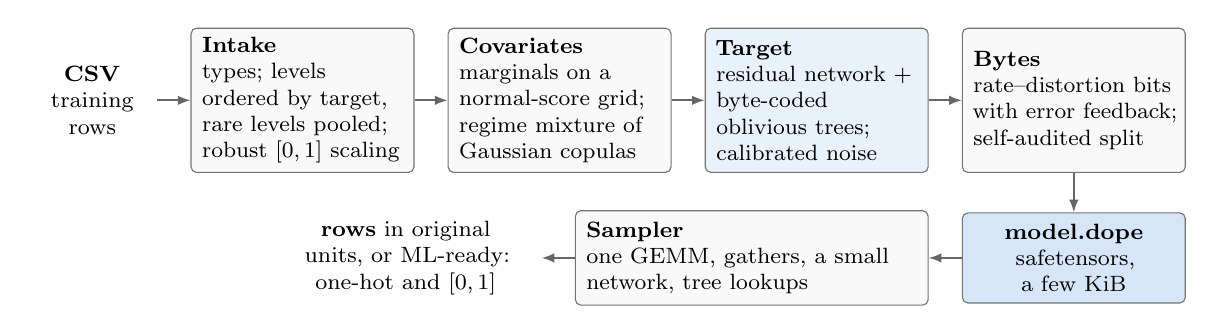
\begin{tikzpicture}[
  font=\footnotesize, node distance=0.42cm,
  stage/.style={draw=stageline, rounded corners=2pt, fill=#1, inner sep=4pt},
  stage/.default=stagefill,
  io/.style={align=center, text width=1.5cm, inner sep=2pt},
  arr/.style={-{Latex[length=1.6mm]}, draw=arrowink, line width=0.6pt}]
  \node[io] (csv) {\textbf{CSV}\\ training rows};
  \node[stage, right=of csv] (intake) {\stagebox{\textbf{Intake}\\ types; levels ordered by target, rare levels pooled; robust $[0,1]$ scaling}};
  \node[stage, right=of intake] (cov) {\stagebox{\textbf{Covariates}\\ marginals on a normal-score grid; regime mixture of Gaussian copulas}};
  \node[stage=targetfill, right=of cov] (tgt) {\stagebox{\textbf{Target}\\ residual network $+$ byte-coded oblivious trees; calibrated noise}};
  \node[stage, right=of tgt] (bytes) {\stagebox{\textbf{Bytes}\\ rate--distortion bits with error feedback; self-audited split}};
  \node[stage=artfill, below=0.5cm of bytes, align=center, text width=\stagewd] (art)
    {\textbf{model.dope}\\ safetensors, a few KiB};
  \node[stage, left=of art, align=left, text width=4.2cm] (smp)
    {\textbf{Sampler}\\ one GEMM, gathers, a small network, tree lookups};
  \node[io, left=of smp, text width=3.3cm] (out) {\textbf{rows} in original units, or ML-ready: one-hot and $[0,1]$};
  \draw[arr] (csv) -- (intake);
  \draw[arr] (intake) -- (cov);
  \draw[arr] (cov) -- (tgt);
  \draw[arr] (tgt) -- (bytes);
  \draw[arr] (bytes) -- (art);
  \draw[arr] (art) -- (smp);
  \draw[arr] (smp) -- (out);
\end{tikzpicture}
\caption{\textbf{A DOPE program, compiled and sampled.} Compilation reads the training rows once; the
artifact stores no rows; sampling reads only the artifact.}
\label{fig:pipeline}
\end{figure}

\paragraph{Intake and ML-ready encoding.}
Column types are inferred from the CSV. A categorical column keeps the levels with at least
\CfgMinLevel{} rows (at most \CfgMaxLevels{}) and pools the rest into an \texttt{\_\_other\_\_} level,
so no singleton label is stored; levels are ordered by their shrunken association with the target
and coded on $[0,1]$, which makes one scalar per categorical column informative for both the copula
and the network. Numeric columns that are non-negative and strongly right-skewed are passed through
$\log(1+x)$, and every numeric column is mapped affinely so that its central ninety-nine percent
spans $[0,1]$; tails are kept inside the program. The same maps produce the ML-ready output that
users request at sampling time: one-hot categorical columns, numeric columns clipped to $[0,1]$ (or
transformed by their own distribution function), and missingness indicators.

\paragraph{Marginals on a normal-score grid.}
Each continuous column stores its quantile function as knots at normal scores $z_k$ evenly spaced
on $[-\CfgZGrid,\CfgZGrid]$, so that $x=Q(\Phi(z))$ is a piecewise-linear function of the latent
score and sampling needs one multiply and one gather per cell. Values repeated in at least
\CfgAtomShare\% of rows are stored as atoms with their score intervals. Columns with at most
\CfgMaxDiscrete{} distinct values, and all categorical columns, are discrete: a draw is the number of
stored thresholds $\Phi^{-1}(F_k)$ that the latent score exceeds.

\paragraph{A regime mixture of Gaussian copulas.}
Dependence lives in normal-score space \citep{sklar1959,nelsen2006copulas}. Scores are van der Waerden
ranks for continuous columns and conditional means $\mathbb{E}[Z\mid\text{level}]$ for discrete ones, whose
correlations are divided by the product of the score standard deviations, a first-order polychoric
correction \citep{olsson1979polychoric}. On top of an independent, Chow--Liu tree
\citep{chow1968dependence}, factor or full correlation model, DOPE fits up to \CfgMaxRegimes{}
\emph{regimes} that share the correlation $R$ but differ in location and scale:
\begin{equation}
  k\sim\mathrm{Cat}(\pi),\qquad z=\mu_k+\sigma_k\odot(M\varepsilon),\qquad x_j=Q_j\!\left(F_j(z_j)\right),
  \qquad F_j(t)=\sum_k \pi_k\,\Phi\!\left(\frac{t-\mu_{kj}}{\sigma_{kj}}\right),
  \label{eq:regimes}
\end{equation}
where $MM^\top=R$ and $\varepsilon\sim\mathcal{N}(0,I)$. Because $F_j(z_j)$ is uniform, every marginal
is reproduced exactly whatever the regimes (supplement); they only shape dependence. A single Gaussian
copula is elliptical in score space, so a table whose rows come from distinct operating modes, with
several columns high together or zero together, is smeared into one ellipse; regimes restore such modes
for about $2d$ bytes each. Regimes are fitted by diagonal
Gaussian-mixture EM \citep{dempster1977em} on the scores, the shared correlation from
within-regime residuals, and the number of regimes (from $\{\CfgRegimeLadder\}$) and the family by
held-out likelihood within the budget. Every family compiles to one mixing matrix $M$, so a draw is
a single matrix product on any device.

\paragraph{The conditional model: a network and a forest.}
The target model has two parts with complementary inductive biases. The first is a residual network
on the $s$ inputs most associated with the target, ranked by the larger of the absolute Spearman
correlation and Chatterjee's $\xi$, which detects non-monotone dependence \citep{chatterjee2021xi}:
\begin{equation}
  \hat y(x)=a+\beta^\top x_c+v^\top\tanh(Wx_c+b),\qquad x_c=x_S-\tfrac12 .
  \label{eq:net}
\end{equation}
For classification the output is a vector of logits. Training uses AdamW
\citep{loshchilov2019adamw} with a cosine schedule while the readout $(a,\beta,v)$, which is linear in a
fixed basis, is periodically replaced by its closed-form ridge or Newton solution
\citep[variable projection;][]{golub1973varpro}; early stopping on an internal validation split picks the
number of steps, so no external data are consulted. Regression noise is a heteroscedastic scale,
log-linear in the leading inputs, times a draw from the stored quantiles of standardized held-out
residuals; class labels are sampled from a softmax whose temperature maximises held-out likelihood
\citep{guo2017calibration}, which by \cref{thm:limit} is the quantity that matters under log-loss.

The network captures smooth and low-order structure in a few hundred bytes. What it misses,
thresholds and interactions among categorical levels, is what tree learners exploit first, and by
\cref{prop:finite} that conditional-mean error enters retention directly. The second part is
therefore a forest of $T$ \emph{oblivious} trees of depth $D$ \citep{prokhorenkova2018catboost} over
all $d$ features, each split being one feature index and one byte:
\begin{equation}
  f_A(x)=\hat y(x)+\sum_{t=1}^{T}\ell_t\Bigl[\textstyle\sum_{l=1}^{D}2^{l-1}\,
  \mathbb{I}\{c(x_{j_{tl}})>\theta_{tl}\}\Bigr],\qquad
  c(x)=\min\bigl(L-1,\max(0,\lfloor(L-1)x+\tfrac12\rfloor)\bigr),
  \label{eq:forest}
\end{equation}
with $L=\CfgLevels$ code levels. Trees are boosted by Newton steps on the loss of the
\emph{quantized} network. Each tree is quantized as soon as it is fitted, to \CfgLeafBits-bit leaf
codes with one half-precision scale, and the next tree is fitted to the gradient of the quantized
ensemble, so rounding errors are corrected by later trees. Depth grows from four to six with the
budget, and the forest kept is the prefix with the lowest validation loss among those that fit the
bytes left; larger budgets therefore buy more trees, and retention keeps rising with bytes instead of
saturating at the network's capacity.

\paragraph{Rate--distortion bit allocation.}
Weights are stored as $b$-bit symmetric integer codes, bit-packed, with one scale per tensor.
\Cref{alg:bits} lowers precision greedily, taking at each step the one-bit reduction with the most
bytes saved per unit of held-out loss, as long as the quantized model keeps all but
$\epsilon=\CfgTolerance\%$ of the stored gain over the null; for distortions that are separable and
convex in the bit depth this greedy path traces the lower convex hull of the rate--distortion curve.
After the hidden layer is quantized, the readout is re-solved on the quantized basis, cancelling most
of the rounding error \citep[an exact form of error feedback;][]{frantar2023gptq}. Marginal knots are eight-bit codes within a half-precision range,
correlations and loadings eight-bit, regime parameters eight-bit on fixed ranges.

\paragraph{Budget search and the self-audit.}
\Cref{alg:compile} spends the budget target-first, as \cref{prop:finite} prescribes: a dependence
model is reserved, the network is sized on a ladder of \CfgPlans{} capacities from \CfgPlanRich{}
to \CfgPlanLean{} (knots, screened inputs, hidden units), the forest takes the bytes left, and any
remainder upgrades the dependence model to the most likely one that fits. One decision is left open
by the theory: how large the reserve should be. \Cref{prop:finite} ranks conditional-mean error first,
but the misspecification remark of \cref{sec:theory} shows that linear and tree auditors also need
covariate structure. DOPE
settles it empirically, without touching test data. For each reserve share in
$\{\CfgShares\}\%$ of the budget it compiles a complete candidate, draws \CfgAuditRows{} rows, trains
fast linear and boosted-tree auditors on them, and keeps the candidate with the highest robust
retention on the compiler's own validation rows. This \emph{self-audit} optimizes the deployment
metric directly, and its value is reported with every artifact. The artifact is a safetensors file with a
single \texttt{U8} tensor: one brotli stream \citep{alakuijala2016brotli} holding the schema, the
structure and every quantized section (supplement); decoding it reproduces exactly the program
evaluated during compilation. Every byte is charged, including the schema, and compressing the schema
together with the codes matters at this scale: inflated, the metadata with column names and category
labels is a median \G{OneMetaShare}\% of a \CfgBudget{} KiB program on the tables of the throughput
study, and the stored stream is a median \G{OneStoredShare}\% of the inflated bytes
(\texttt{--anonymize} replaces names and labels by codes). The default budget is \CfgBudget{} KiB.

\begin{algo}[t]
\caption{\textsc{Compile}$(D_{\mathrm{fit}}, B)$: target-first program search within $B$ bytes.}
\label{alg:compile}
\small
\begin{enumerate}[leftmargin=2em,itemsep=1pt,topsep=3pt,label=\arabic*:]
\item Infer the schema; order and pool category levels; scale numeric columns; hold out validation rows.
\item Fit marginals on the normal-score grid; compute latent scores and their corrected correlation $R$.
\item Fit regimes $K\in\{\CfgRegimeLadder\}$ and every dependence family; rank each pair by held-out likelihood.
\item Rank inputs by $\max\{|\rho_{\mathrm{S}}|,\xi\}$ with the target.
\item \textbf{for} each reserve share $\sigma$ \textbf{do}
\item \hspace{1.2em}reserve the most likely dependence model costing at most $\sigma B$;
\item \hspace{1.2em}\textbf{for} up to three capacities $(m,s,h)$ spread down the ladder that fit \textbf{do}
\item \hspace{2.4em}train \eqref{eq:net} with closed-form readouts; allocate bits by \cref{alg:bits};
\item \hspace{2.4em}boost trees \eqref{eq:forest} on the quantized network; keep the best prefix that fits $B$;
\item \hspace{1.2em}keep the smallest capacity unless a larger one lowers held-out loss by a clear margin;
\item \hspace{1.2em}upgrade dependence to the most likely model that fits; self-audit the candidate.
\item Return the candidate with the highest self-audited robust retention, decoded from its artifact.
\end{enumerate}
\end{algo}

\begin{algo}[t]
\caption{Rate--distortion bit allocation with error feedback.}
\label{alg:bits}
\small
\begin{enumerate}[leftmargin=2em,itemsep=1pt,topsep=3pt,label=\arabic*:]
\item Start every weight tensor at eight bits; let $G$ be the stored gain over the null on validation rows.
\item \textbf{repeat}: for each tensor, quantize it one bit coarser, re-solve the readout on the quantized basis,
  and measure the validation loss;
\item \hspace{1.2em}take the step with the most bytes saved per unit of added loss, provided the total added loss stays within $\epsilon G$;
\item \textbf{until} no step qualifies. Return the codes and per-tensor scales.
\end{enumerate}
\end{algo}

\paragraph{Sampling.}
A draw is a short tensor program: counter-based normal and uniform inputs (so a seed fixes the rows), $z=M\varepsilon$, a regime gather, per-column gathers on the knot grids, a
missingness mask, the network \eqref{eq:net}, one comparison per tree level and one leaf gather per
tree \eqref{eq:forest}, and the noise. Its cost is $O(N(dm+Kd+sh+TD))$ time and $O(|A|)$ memory; at the default budget the program is small enough to stay in a core's L1 cache.
On CPU the draw is evaluated row by row in parallel; the CUDA and Metal builds run it as candle tensors
but are not tested in this paper.

\section{Experiments}
\label{sec:experiments}

\paragraph{Tables and protocol.}
We use \G{OneTables} public tables from UCI \citep{kelly2023uci} and PMLB \citep{olson2017pmlb}: classification
(adult, bank marketing, credit default, German credit, car evaluation, mushroom, covertype) and
regression (California housing, abalone, wine quality, bike sharing, concrete, airfoil, energy,
student performance, online news), mixed numeric and categorical, with missing values where the
source has them. Each table is split into training and test rows (stratified for classification),
capped at \CfgMaxTrain{} training and \CfgMaxTest{} test rows. Every method sees only the training
rows. Synthetic tables have as many rows as the real training split. Auditors are ridge or logistic
regression, CatBoost \citep{prokhorenkova2018catboost} with \CfgCatIters{} trees of depth \CfgCatDepth{},
and a two-layer MLP \citep{pedregosa2011sklearn}, each fitted with its own one-hot encoding and scaling.
A fit that fails, for instance because a table's schema alone exceeds the budget, or that exceeds the
wall-clock limit counts as robust retention zero, the null fallback. Per table we take the median over
three seeds for DOPE and compressed rows at the default budget, the research kernel, the Gaussian
copula and ARF; every other cell, including the other budgets and the ablations, has one seed. Across tables we report medians with percentile bootstrap
intervals (\CfgDraws{} draws over tables) and paired differences as Hodges--Lehmann estimates.

\paragraph{Comparators.}
The \emph{information-compression control} answers the question a skeptic should ask first: why not
ship the data? For each budget it keeps the largest random subset of real training rows whose CSV,
compressed with xz at its strongest preset, fits the budget; auditors train on those real rows as
they are. We also run the SDV Gaussian copula \citep{patki2016sdv}, ARF \citep{watson2023arf}, and on the
tables with at most a few thousand training rows CTGAN and TVAE \citep{xu2019ctgan}, all at their
defaults; their bytes are the xz-compressed pickles of the fitted objects, which favours them. The
repository's \emph{research kernel}, an earlier DOPE engine with a fixed program shape
(\texttt{dope-kernel fit-table} at its defaults), is run on every table; it accepts regression and
binary targets only, so it refuses one multiclass table and fits the other's class codes as a
regression, and both count as measured. Real rows resampled with replacement are a row-count control,
not a generator and not a ceiling.

\begin{table}[t]
\centering
\caption{\textbf{Main results.} Median over tables of robust retention with its \CfgConf\% bootstrap
interval, the median retention of each auditor family, and the number of tables whose robust retention
reaches $\tau$. Bytes are medians of everything sampling reads (DOPE and the kernel: the artifact file;
real rows: the xz stream; generators: xz-compressed pickles). A superscript gives the table count when a method
covers fewer tables.}
\label{tab:main}
\small
\IfFileExists{generated/dope1-table.tex}{\resizebox{\linewidth}{!}{\begin{tabular}{lrrrrrr}
\toprule
Method & Bytes & Robust retention [95\% CI] & Linear & CatBoost & MLP & $\geq 0.9$ \\
\midrule
DOPE, 2 KiB & 2.0~KiB & 0.905 [0.81, 0.94] & 0.94 & 0.93 & 0.94 & 8/16 \\
\textbf{DOPE, 4 KiB (default)} & 3.8~KiB & 0.909 [0.84, 0.93] & 0.96 & 0.94 & 0.93 & 9/16 \\
DOPE, 16 KiB & 5.7~KiB & 0.933 [0.87, 0.97] & 0.96 & 0.95 & 0.95 & 10/16 \\
DOPE, 64 KiB & 9.6~KiB & 0.930 [0.88, 0.96] & 0.96 & 0.95 & 0.97 & 11/16 \\
DOPE research kernel & 1.1~KiB & 0.677 [0.48, 0.84] & 0.95 & 0.79 & 0.82 & 3/16 \\
\midrule
Real rows (xz), 4 KiB & 4.0~KiB & 0.340 [\ensuremath{-}4.01, 0.92] & 0.94 & 0.87 & 0.38 & 5/16 \\
Real rows (xz), 64 KiB & 50.8~KiB & 0.983 [0.95, 1.00] & 1.00 & 1.00 & 0.98 & 12/16 \\
Real rows (xz), all & 52.2~KiB & 0.999 [1.00, 1.00] & 1.00 & 1.00 & 1.00 & 16/16 \\
\midrule
Gaussian copula (SDV) & 82.0~KiB & 0.282 [0.09, 0.45] & 0.76 & 0.40 & 0.29 & 1/16 \\
ARF & 673.1~KiB & 0.705 [0.00, 0.86] & 0.94 & 0.85 & 0.85 & 3/16 \\
TVAE (SDV)$^{7}$ & 247.7~KiB & \ensuremath{-}0.460 [\ensuremath{-}1.36, 0.61] & 0.73 & 0.40 & \ensuremath{-}0.53 & 0/7 \\
CTGAN (SDV)$^{7}$ & 712.9~KiB & \ensuremath{-}1.897 [\ensuremath{-}3.06, \ensuremath{-}0.47] & \ensuremath{-}0.18 & \ensuremath{-}0.39 & \ensuremath{-}2.33 & 0/7 \\
Real rows, resampled & 52.1~KiB & 0.929 [0.67, 0.99] & 1.00 & 0.97 & 0.96 & 9/16 \\
\bottomrule
\end{tabular}
}}{\pending{main table}}
\end{table}

\paragraph{Predictive structure per byte.}
\Cref{fig:frontier,tab:main} give the main result. At its default budget DOPE's program has a median
size of \G{OneDopeCBytes} and a median robust retention of \G{OneDopeCRet}
[\G{OneDopeCLo}, \G{OneDopeCHi}], with \G{OneDopeCReach} of \G{OneDopeCN} tables at or above $\tau$.
Spending the same budget on real rows gives \G{OneRowsCRet}: the few hundred rows that fit train linear
models and CatBoost (\G{OneRowsCLin} and \G{OneRowsCCb}) but not the MLP (\G{OneRowsCMlp}), and the robust
score keeps the worst family, whereas the program generates as many rows as wanted from the structure
it stores. \Cref{fig:tables} shows every table and \cref{tab:equal} pairs the two at every
budget. Half the default budget already suffices: there DOPE reaches \G{OneDopeBRet}
[\G{OneDopeBLo}, \G{OneDopeBHi}] and beats compressed rows with wins, ties and losses \G{OneEqBWtl}
(sign test $p=\G{OneEqBP}$). Wherever DOPE fits the budget, it wins \G{OneEqWins} and loses
\G{OneEqLosses} of \G{OneEqCells} paired comparisons; it does not fit within the smallest budget on
\G{OneDopeFailedA} tables, whose schema with its column names and category labels and the leanest
program already exceed it. Compressed rows overtake
DOPE once the budget holds a large share of a table: they need \G{OneRowsFBytes} to reach
\G{OneRowsFRet}, and the whole table (\G{OneRowsFullBytes}) to reach \G{OneRowsFullRet}.
The generators sit far to the right: the Gaussian copula reaches \G{OneCopulaRet} at
\G{OneCopulaBytes} and ARF \G{OneArfRet} at \G{OneArfBytes}.

\paragraph{Against the research kernel.}
The repository's earlier engine compiles programs of one fixed shape, a median \G{OneKernelBytes},
and reaches \G{OneKernelRet} [\G{OneKernelLo}, \G{OneKernelHi}]. Its linear auditors keep
\G{OneKernelLin} but CatBoost only \G{OneKernelCb}: without trees its program misses the thresholds
and interactions that tree auditors exploit, as the no-trees ablation below shows for DOPE. On the
\G{OneKernelSupported} regression and binary tables it supports, DOPE at the smallest budget, about the
kernel's size, cannot be separated from it (wins, ties and losses \G{OneKernelVsAWtl}; Hodges--Lehmann difference
\G{OneKernelVsAHl} [\G{OneKernelVsALo}, \G{OneKernelVsAHi}]); at half the default budget it is ahead
(\G{OneKernelVsBWtl}; \G{OneKernelVsBHl} [\G{OneKernelVsBLo}, \G{OneKernelVsBHi}]), and at the
default budget \G{OneKernelVsCWtl}.

\begin{table}[t]
\centering
\caption{\textbf{Equal bytes.} Median robust retention of DOPE and of real training rows compressed with
xz to the same budget, over the tables where both ran and DOPE fitted within the budget, with paired
wins, ties and losses, an exact sign test, and the number of tables on which DOPE did not fit.}
\label{tab:equal}
\small
\IfFileExists{generated/dope1-equalbytes.tex}{\begin{tabular}{lrrrrrr}
\toprule
Budget & Tables & DOPE & Real rows (xz) & DOPE wins/ties/losses & Sign test $p$ & DOPE did not fit \\
\midrule
1~KiB & 12 & 0.797 & \ensuremath{-}0.409 & 11/0/1 & 0.0063 & 4 \\
2~KiB & 16 & 0.905 & \ensuremath{-}0.286 & 14/0/2 & 0.0042 & 0 \\
4~KiB & 16 & 0.909 & 0.340 & 11/0/5 & 0.21 & 0 \\
8~KiB & 16 & 0.939 & 0.564 & 10/0/6 & 0.45 & 0 \\
16~KiB & 16 & 0.933 & 0.872 & 10/0/6 & 0.45 & 0 \\
64~KiB & 16 & 0.930 & 0.983 & 4/0/12 & 0.077 & 0 \\
\bottomrule
\end{tabular}
}{\pending{equal-bytes table}}
\end{table}

\begin{figure}[t]
  \centering
  \GeneratedFigure[\tallwidth]{dope1-tables.pdf}{per-table equal-bytes comparison}
  \caption{\textbf{Every table at the default budget.} Robust retention of DOPE (blue) and of real
  training rows compressed with xz to the same bytes (orange; a triangle marks a value below the axis).
  The dotted line is $\tau$.}
  \label{fig:tables}
\end{figure}

\begin{figure}[t]
  \centering
  \GeneratedFigure[\herowidth]{dope1-coverage.pdf}{TDL coverage curves}
  \caption{\textbf{Transfer Description Length.} Share of tables whose robust retention reaches $\tau$
  (solid) or a lower threshold (dashed) within a given number of bytes, for DOPE and for xz-compressed
  real rows. Each step is one table's TDL.}
  \label{fig:coverage}
\end{figure}

\paragraph{TDL.}
\Cref{fig:coverage} turns the frontier into the KPI. DOPE reaches $\tau$ on \G{OneTdlDopeN} of
\G{OneTables} tables, at a median TDL of \G{OneTdlDopeMedian}; compressed real rows reach it on
\G{OneTdlRowsN}, at a median of \G{OneTdlRowsMedian}, by keeping a large part of the table. At the
lower threshold the counts are \G{OneTdlDopeEightyN} and \G{OneTdlRowsEightyN}. The supplement lists
every table; the ones DOPE does not bring to $\tau$ within the tested budgets are those whose
retention keeps rising for compressed rows but saturates for the program, so they mark where a richer
conditional model, rather than more bytes of the same model, is needed.

\begin{table}[t]
\centering
\caption{\textbf{Ablations at the default budget and seed.} Each row removes or changes one component
of DOPE; the last column counts the tables on which the variant beats, ties or trails the full program.}
\label{tab:ablation}
\small
\IfFileExists{generated/dope1-ablation.tex}{\resizebox{\linewidth}{!}{\begin{tabular}{lrrrrrr}
\toprule
Variant (4 KiB, seed 0) & Bytes & Robust retention [95\% CI] & Linear & CatBoost & MLP & Better/tied/worse \\
\midrule
DOPE (default) & 3.8~KiB & 0.919 [0.83, 0.95] & 0.95 & 0.95 & 0.96 & -- \\
independent features, one regime & 3.3~KiB & 0.798 [0.54, 0.89] & 0.85 & 0.89 & 0.92 & 4/0/12 \\
one regime (plain Gaussian copula) & 3.4~KiB & 0.835 [0.76, 0.93] & 0.91 & 0.92 & 0.93 & 4/1/11 \\
network only, no trees & 1.6~KiB & 0.862 [0.77, 0.94] & 0.98 & 0.88 & 0.93 & 1/0/15 \\
linear target model, no trees & 1.0~KiB & 0.593 [0.37, 0.80] & 0.96 & 0.62 & 0.77 & 3/0/13 \\
fixed byte split, no self-audit & 3.8~KiB & 0.919 [0.83, 0.95] & 0.95 & 0.95 & 0.96 & 1/14/1 \\
four times as many synthetic rows & 3.8~KiB & 0.944 [0.81, 0.95] & 0.96 & 0.97 & 0.97 & 11/0/5 \\
\bottomrule
\end{tabular}
}}{\pending{ablation table}}
\end{table}

\paragraph{What each component buys.}
\Cref{tab:ablation} removes one component at a time at the default budget and seed, where the full
program reaches \G{OneDopeSeedZeroRet}; the last column counts the tables on which the variant is better,
tied or worse. Without trees, the network alone reaches \G{OneDopeNoTreesRet} (better, tied or worse on
\G{OneAblDopeNoTreesWtl} tables), and a linear target
model without trees \G{OneDopeLinearRet}: the forest carries the thresholds and interactions that tree
auditors exploit. Sampling features independently, while keeping the conditional model, gives
\G{OneDopeIndepRet}: linear and tree auditors need the joint covariate structure, as the
misspecification remark in \cref{sec:theory} predicts. A single regime gives \G{OneDopeOneRegimeRet}.
A fixed byte split without the self-audit gives \G{OneDopeNoAuditRet} (better, tied or worse on
\G{OneAblDopeNoAuditWtl} tables): the self-audit rarely changes which program is kept, and its main
value is the retention estimate it reports with every artifact. Drawing four times as many rows
from the same program gives \G{OneDopeFourRet}; the MLP auditor also switches solver on larger training
sets, so we do not attribute this gain to the program.

\paragraph{Compute.}
Compilation, including the self-audit, takes a median of \G{OneDopeCFit} per table at the default
budget on a two-core machine, against \G{OneCopulaFit} for the Gaussian copula and \G{OneArfFit}
for ARF. Writing synthetic rows to CSV, end to end, runs at a median of \G{OneDopeCRate} rows per
second; the in-memory sampler is measured separately with the engine CLI's \texttt{throughput} command
(\texttt{engine/target/release/dope throughput}; supplement).
A draw touches only a few kilobytes of parameters, but its cost grows with the number of trees, so
the largest programs sample several times more slowly than the default one; sampling scales with
cores; the GPU path is built but not measured here.

\paragraph{The self-audit predicts retention.}
Over all \G{OneAuditN} fitted DOPE programs, the self-audited retention that the compiler reports,
computed only from the training rows, ranks programs like the measured robust retention on held-out
test rows (Spearman \G{OneAuditRho}), with a median absolute difference of \G{OneAuditMae} and a
median bias of \G{OneAuditBias} (supplement). A user therefore learns at compile time, without
test data, roughly how much predictive structure a program keeps.

\paragraph{Per family.}
DOPE's median retention is \G{OneDopeCLin} for linear auditors, \G{OneDopeCCb} for CatBoost and
\G{OneDopeCMlp} for MLPs, so boosted trees, which exploit the finest interactions, usually set its
robust score. For compressed real rows at the same budget the limiting family is the MLP
(\G{OneRowsCMlp}, against \G{OneRowsCCb} for CatBoost): a network trained on a few hundred rows
overfits, and its log-loss on test rows can be far worse than the null.

\section{Related work}
\label{sec:related}

\paragraph{Generators.} Copulas and Bayesian networks \citep{patki2016sdv,chow1968dependence,aas2009paircopula,zhang2014privbayes}
fit explicit, often small, joint models; adversarial and variational models \citep{xu2019ctgan},
diffusion models \citep{kotelnikov2023tabddpm,zhang2024tabsyn,shi2025tabdiff}, forests
\citep{watson2023arf,jolicoeurmartineau2024forestdiffusion}, language models \citep{borisov2023great} and
prior-fitted networks \citep{hollmann2025tabpfn} model the joint table with many parameters
\citep{borisov2024survey}. DOPE targets the conditional model explicitly, keeps the covariate model
small, and is charged for every byte.

\paragraph{Evaluation.} Train-on-synthetic, test-on-real evaluation goes back to \citet{esteban2017rcgan};
\citet{jordon2018measuring} ask whether synthetic data preserve the ranking of learners, and utility and
fidelity measures and suites broaden the picture \citep{snoke2018utility,alaa2022faithful,qian2023synthcity,erickson2026tabarena}.
Retention is a null-normalized TSTR/TRTR ratio; what is new here is its information-theoretic reading,
the worst case over model families, and the byte axis with an equal-byte real-row control.

\paragraph{Compression and distillation.} Dataset distillation keeps a few training examples and model
distillation keeps a model's behaviour \citep{wang2018distillation,hinton2015distilling}; generative
compression names learned media codecs \citep{santurkar2017generative}; description-length and
bottleneck ideas \citep{rissanen1978modeling,blumer1987occam,tishby2000bottleneck} motivate the framing.
DOPE ships a program that draws fresh rows, and TDL charges it in bytes against a downstream
distortion.

\paragraph{Privacy.} Membership and attribute attacks on synthetic data
\citep{shokri2017membership,stadler2022groundhog,vanbreugel2023domias} and holdout-referenced distances
\citep{platzer2021holdout} are empirical; formal differential privacy \citep{dwork2014foundations} requires
a mechanism. DOPE stores no rows, but an artifact keeps column names, category labels
and quantiles unless \texttt{--anonymize} replaces them with codes, and this paper makes no privacy claim.

\section{Limitations}
\label{sec:limits}

The panel is public, and its tables are smaller and better curated than many private ones. The
retention gate is measured with point estimates per table; the contract's lower confidence bound and
the driver-agreement gate are not measured here, and foundation-model auditors are not yet included.
Large neural generators (TabSyn, TabDDPM, TabDiff) were not run, CTGAN and TVAE ran only on the
smaller tables, and fits over the wall-clock limit count as failures. Every result is measured on CPU;
the CUDA and Metal backends are built but not tested. The evaluation is not sealed, so every result
here is selection-exposed validation. A development panel of other tables guided most engineering
choices, but the forest and the self-audit were added after an earlier engine had been scored on three
of the confirmation tables (adult, airfoil and abalone). The compact container, which stores the schema
and the codes as one compressed stream, and the regrowth of trees into the bytes it saves were added
after a first full run of the whole panel showed that plain header text took most of a default
artifact. These changes alter how a program is stored and how many trees fit a budget, not how anything
is fitted; every DOPE cell was re-run, and the superseded records are kept in the repository. Each program serves one declared target. Columns that are exact functions of one
another, such as an education level and its numeric code, are kept only as strongly dependent, not as
identical. This paper runs no privacy attacks; DOPE is not a formal
differential-privacy mechanism and not HIPAA de-identification.

\section{Conclusion}

A few kilobytes of the right structure train models nearly as well as the table they came from, and
at the smallest budgets better than the same bytes spent on the rows themselves (wins, ties and losses
\G{OneEqAWtl} at the smallest budget and \G{OneEqBWtl} at half the default). Retention measures how much of a table's
predictive information survives, TDL measures what that costs in bytes, and DOPE is a program that
spends its bytes where the theory says they count. The engine, the benchmark records and the scripts
that regenerate every number in this paper are open.


\bibliographystyle{plainnat}
\bibliography{references,references-dope1}
\end{document}
